% !TeX program = xelatex
% ============================================================
% 2010 年·普通高等学校招生考试·重庆卷·文科 · 试题版
% 由 tools/make_editions.py 生成（重跑会覆盖本文件）；
% 题目/解析内容在 questions.tex / answers*.tex，勿在本文件内写内容。
% ============================================================
\documentclass[zihao=-4, a4paper]{ctexart}
% ============================================================
% common/preamble.tex —— 拆分版试卷项目 · 公共导言区
% 引擎：XeLaTeX；文档类 ctexart 由各版本壳文件自行声明
% 由合并书 math-gaokao-2017-2026/preamble.tex 改造而来：
%   - 页眉左右改为可重定义宏 \gkheadL / \gkheadR（各版本壳设置）
%   - hyperref 不再写死 pdftitle（壳内 \hypersetup 覆盖）
%   - 删除书籍专用的 \chaptermark 重定义与 \gkpaper 装配宏
% ============================================================

% ---------- 数学 ----------
\usepackage{amsmath}
\usepackage{amssymb}
\usepackage{mathtools}

% ---------- 绘图 ----------
\usepackage{tikz}
\usetikzlibrary{shapes.geometric, arrows.meta, calc, patterns, angles, quotes, positioning}
\usepackage{pgfplots}
\pgfplotsset{compat=1.18}

% ---------- 版面 ----------
\usepackage{geometry}
\usepackage{needspace}
\geometry{a4paper, margin=2.2cm, headheight=15pt}
% 紧凑版式（如印刷版）可在壳文件中于 \begin{document} 前再次调用 \geometry 覆盖
\usepackage{enumitem}
\setlist{itemsep=2pt, topsep=4pt, parsep=0pt}

% 中文与行内公式混排的断行弹性：
% emergencystretch 允许段落末路不通时追加伸展量；
% 降低二元/关系符罚分，允许行内长公式在 = 、+ 等处断行（否则整段外溢）
\emergencystretch=2em
\binoppenalty=700
\relpenalty=500
\usepackage{booktabs}      % 三线表
\usepackage[most]{tcolorbox}

% ---------- 选择题选项对齐 ----------
% tasks 宏包：\begin{gkopts}(列数) \task ... \end{gkopts}
% 自动等宽分栏，选项天然对齐；列数已由内容片段按选项长度写定（4/2/1）
\usepackage{tasks}
\settasks{label={}, label-width=0pt, item-indent=1.2em,
          column-sep=1em, after-item-skip=2pt, before-skip=2pt, after-skip=4pt}
\NewTasksEnvironment[style=itemize]{gkopts}[\task](4)

% ---------- 页眉页脚 ----------
\newcommand{\gkheadL}{}   % 左页眉：卷名（壳文件 \renewcommand 设置）
\newcommand{\gkheadR}{}   % 右页眉：版本名（壳文件 \renewcommand 设置）
\usepackage{fancyhdr}
\pagestyle{fancy}
\fancyhf{}
\fancyhead[L]{\small\gkheadL}
\fancyhead[R]{\small\gkheadR}
\fancyfoot[C]{\small —— 第 \thepage\ 页 ——}
\renewcommand{\headrulewidth}{0.4pt}

% ---------- 超链接（须最后加载）----------
\usepackage{hyperref}
\hypersetup{colorlinks=true, linkcolor=blue!55!black,
            bookmarksnumbered=true, unicode=true}

% ============================================================
% common/macros.tex —— 自定义命令与环境（题号、解析头、提示框等）
% 与合并书 math-gaokao-2017-2026/preamble.tex 的自定义段保持一致，
% 保证内容片段（questions.tex / answers.tex）在两个项目间可互换。
% ============================================================

% ---------- 试卷标识（壳文件 \renewcommand 设置，用于 label 命名空间）----------
\newcommand{\gkpaperid}{none}

% ---------- 题号 ----------
% 试题部分的题号：加粗编号 + 自动 \label{q:<卷id>:<题号>}
\newcommand{\gkti}[1]{\par\medskip\noindent
  \textbf{#1．}\phantomsection\label{q:\gkpaperid:#1}\ignorespaces}
% 多卷/分部重启题号时，#1 是唯一内部顺序号（交叉引用身份），#2 才是原卷显示题号。
\newcommand{\gktiwithlabel}[2]{\par\medskip\noindent
  \textbf{#2．}\phantomsection\label{q:\gkpaperid:#1}\ignorespaces}

% 解析部分的题头：小标题 + 回链到试题页
% （仅在题目与解析同文档的版本中回链有效；试题版不含解析头，无悬空引用）
\newcommand{\gksolhead}[2]{%
  \Needspace{3\baselineskip}\subsubsection*{第 #1 题\if\relax\detokenize{#2}\relax\else（#2）\fi}%
  \phantomsection\label{s:\gkpaperid:#1}%
  {\small\color{gray}（题目见第~\pageref{q:\gkpaperid:#1}~页）}\par\nopagebreak}
% 与 \gktiwithlabel 成对：显示原题号，但回链仍用唯一内部顺序号。
\newcommand{\gksolheadwithlabel}[3]{%
  \Needspace{3\baselineskip}\subsubsection*{第 #2 题\if\relax\detokenize{#3}\relax\else（#3）\fi}%
  \phantomsection\label{s:\gkpaperid:#1}%
  {\small\color{gray}（题目见第~\pageref{q:\gkpaperid:#1}~页）}\par\nopagebreak}

% ---------- 填空题空位 ----------
\newcommand{\gkblank}{\underline{\hspace{2.2em}}}

% ---------- 提示框 ----------
% 卷种提示 / 解析归属声明（醒目，浅黄）
\newtcolorbox{gknotice}{colback=yellow!8, colframe=orange!60!black,
  boxrule=0.5pt, arc=1.5pt, left=6pt, right=6pt, top=4pt, bottom=4pt,
  before skip=8pt, after skip=8pt}

% 方法提示 / 注（浅蓝，用于解析后的点评与题量说明）
\newtcolorbox{gktip}{colback=blue!4, colframe=blue!35!black,
  boxrule=0.4pt, arc=1.5pt, left=6pt, right=6pt, top=4pt, bottom=4pt,
  before skip=6pt, after skip=6pt, fontupper=\small}

% ---------- 答案行 ----------
% 解析中独立成段的"答案：X"用带底色的行呈现
\newcommand{\gkanswer}[1]{\par\smallskip\noindent
  \tcbox[width=\linewidth, tcbox width=auto limited,
         colback=green!6, colframe=green!35!black, boxrule=0.4pt,
         arc=1.5pt, left=4pt, right=4pt, top=2pt, bottom=2pt,
         nobeforeafter]{\textbf{#1}}\par\smallskip}

% ---------- 结构标题 ----------
% 结构标题后通常紧跟一个带 0.5\textheight 起始预留的解析题块；0.4 只够放标题，
% 会把下一题整体推到下一页，留下孤立的「二、填空题」等页尾标题。
\newcommand{\gkpart}[1]{\Needspace{0.6\textheight}\subsection*{#1}\nopagebreak}     % 标题 + 首题
% （一）必考题 / 解析小问标题：块式加粗段，可自动换行（\paragraph 的 run-in 版式会溢出）
\newcommand{\gksubpart}[1]{\Needspace{6\baselineskip}\par\medskip\noindent\textbf{#1}\par\nopagebreak\smallskip}

% 罗马数字Ⅰ-Ⅻ（U+2160）与圈号①②③（U+2460）划入 CJK 字符类，
% 用中文字体渲染——西文字体 Latin Modern 缺这些字形，否则整段静默丢字
\xeCJKDeclareCharClass{CJK}{"2160 -> "217F, "2460 -> "24FF}

% ============================================================
% common/questions_env.tex —— 题目 / 解析的语义包装环境
%
% questions.tex 中每道题包在 \begin{question}...\end{question} 里，
% answers.tex 中每题解析包在 \begin{answer}...\end{answer} 里；
% 题头排版仍由内容行中的 \gkti / \gksolhead 完成（见 macros.tex）。
%
% 环境本身不产生任何盒子或垂直间距（只引入一个 TeX 分组），
% 排版结果与不包裹时逐点一致。它的价值在于：
%   1. 给每道题一个机器可数的结构边界（校验脚本数环境数 = 题量）；
%   2. 为将来的条件编译留钩子——某版本可重定义环境实现按题取舍。
% ============================================================

% 环境不把整题装盒：题目与解析仍可自然跨页，但开始题块前必须为题面、
% 图形/表格或解析首段留出足够空间。仅保留 2 个 baseline 会让题干、
% 选项和图形在页边界处被拆开，形成不可打印的孤立内容；题目保留
% 0.15\textheight，在避免短题制造大段空白与避免题块拆分之间取平衡。
% 解析题块保留 0.5\textheight，以容纳“题面 + 图形/选项 + 首段解析”；
% 结构标题仍用更大的保留量；末页自然收尾由视觉复审判定。
\newenvironment{question}{\Needspace{0.15\textheight}}{}
\newenvironment{answer}{\Needspace{0.5\textheight}}{}

\renewcommand{\gkpaperid}{gk-2010-chongqing-arts}
\renewcommand{\gkheadL}{2010 年·普通高等学校招生考试·重庆卷·文科 · 数学}
\renewcommand{\gkheadR}{试题版}
\hypersetup{pdftitle={2010 年·普通高等学校招生考试·重庆卷·文科 数学 · 试题版}}
\begin{document}
\begin{center}
  {\Large\bfseries 2010 年·普通高等学校招生考试·重庆卷·文科}\\[4pt]
  {\large 数学 · 试题版}
\end{center}
\medskip
\pdfbookmark[1]{试题}{sec:q}
% questions.tex —— 2010 年·普通高等学校招生考试·重庆卷·文科 · 题目内容片段（无答案）
% 由 tools/generate_projects.py 依来源总账自 2010/2010_数学真题_重庆文_试题.md 生成，勿手改（改源 MD 后重跑）
状态：needs-review；依固定候选 PDF 两页（印刷页 579–580）逐题核验，三幅图已矢量重绘。原页未印分值，不补。
\gkpart{一、选择题}
\begin{question}
\gkti{1}$(x+1)^4$ 的展开式中 $x^2$ 的系数为（　）

（A）$4$

（B）$6$

（C）$10$

（D）$20$

\end{question}
\begin{question}
\gkti{2}在等差数列 $\{a_n\}$ 中，$a_1+a_9=10$，则 $a_5$ 的值为（　）

（A）$5$

（B）$6$

（C）$8$

（D）$10$

\end{question}
\begin{question}
\gkti{3}若向量 $\boldsymbol a=(3,m)$，$\boldsymbol b=(2,-1)$，$\boldsymbol a\cdot\boldsymbol b=0$，则实数 $m$ 的值为（　）

（A）$-\dfrac32$

（B）$\dfrac32$

（C）$2$

（D）$6$

\end{question}
\begin{question}
\gkti{4}函数 $y=\sqrt{16-4^x}$ 的值域是（　）

（A）$[0,+\infty)$

（B）$[0,4]$

（C）$[0,4)$

（D）$(0,4)$

\end{question}
\begin{question}
\gkti{5}某单位有职工 $750$ 人，其中青年职工 $350$ 人，中年职工 $250$ 人，老年职工 $150$ 人，为了了解该单位职工的健康情况，用分层抽样的方法从中抽取样本。若样本中的青年职工为 $7$ 人，则样本容量为（　）

（A）$7$

（B）$15$

（C）$25$

（D）$35$

\end{question}
\begin{question}
\gkti{6}下列函数中，周期为 $\pi$，且在 $\left[\dfrac{\pi}{4},\dfrac{\pi}{2}\right]$ 上为减函数的是（　）

（A）$y=\sin\left(2x+\dfrac{\pi}{2}\right)$

（B）$y=\cos\left(2x+\dfrac{\pi}{2}\right)$

（C）$y=\sin\left(x+\dfrac{\pi}{2}\right)$

（D）$y=\cos\left(x+\dfrac{\pi}{2}\right)$

\end{question}
\begin{question}
\gkti{7}设变量 $x$，$y$ 满足约束条件
\nopagebreak[4]
\[\begin{cases}x\geqslant 0,\\x-y\geqslant 0,\\2x-y-2\leqslant 0,\end{cases}\]
则 $z=3x-2y$ 的最大值为（　）

（A）$0$

（B）$2$

（C）$4$

（D）$6$

\end{question}
\begin{question}
\gkti{8}若直线 $y=x-b$ 与曲线
\nopagebreak[4]
\[\begin{cases}x=2+\cos\theta,\\y=\sin\theta,\end{cases}\quad(\theta\in[0,2\pi))\]
有两个不同的公共点，则实数 $b$ 的取值范围为（　）

（A）$(2-\sqrt2,1)$

（B）$[2-\sqrt2,2+\sqrt2]$

（C）$(-\infty,2-\sqrt2)\cup(2+\sqrt2,+\infty)$

（D）$(2-\sqrt2,2+\sqrt2)$

\end{question}
\begin{question}
\gkti{9}到两互相垂直的异面直线的距离相等的点（　）

（A）只有 $1$ 个

（B）恰有 $3$ 个

（C）恰有 $4$ 个

（D）有无穷多个

\end{question}
\begin{question}
\gkti{10}某单位拟安排 $6$ 位员工在今年 $6$ 月 $14$ 日至 $16$ 日（端午节假期）值班，每天安排 $2$ 人，每人值班 $1$ 天。若 $6$ 位员工中的甲不值 $14$ 日，乙不值 $16$ 日，则不同的安排方法共有（　）

（A）$30$ 种

（B）$36$ 种

（C）$42$ 种

（D）$48$ 种

\end{question}
\gkpart{二、填空题}
\begin{question}
\gkti{11}设 $A=\{x\mid x+1>0\}$，$B=\{x\mid x<0\}$，则 $A\cap B=$ $\underline{\qquad}$。

\end{question}
\begin{question}
\gkti{12}已知 $t>0$，则函数 $y=\dfrac{t^2-4t+1}{t}$ 的最小值为 $\underline{\qquad}$。

\end{question}
\begin{question}
\gkti{13}已知过抛物线 $y^2=4x$ 的焦点 $F$ 的直线交该抛物线于 $A$、$B$ 两点，$|AF|=2$，则 $|BF|=$ $\underline{\qquad}$。

\end{question}
\begin{question}
\gkti{14}加工某一零件需经过三道工序，设第一、二、三道工序的次品率分别为 $\dfrac{1}{70}$、$\dfrac{1}{69}$、$\dfrac{1}{68}$，且各道工序互不影响，则加工出来的零件的次品率为 $\underline{\qquad}$。

\Needspace{0.4\textheight}
\end{question}
\begingroup
\renewenvironment{question}{\Needspace{0.5\textheight}}{}
\begin{question}
\gkti{15}如图，图中的实线是由三段圆弧连接而成的一条封闭曲线 $C$，各段弧所在的圆经过同一点 $P$（点 $P$ 不在 $C$ 上）且半径相等。设第 $i$ 段弧所对的圆心角 $\alpha_i$（$i=1,2,3$），则 $\cos\dfrac{\alpha_1}{3}\cos\dfrac{\alpha_2+\alpha_3}{3}-\sin\dfrac{\alpha_1}{3}\sin\dfrac{\alpha_2+\alpha_3}{3}=$ $\underline{\qquad}$。
\nopagebreak[4]
\begin{center}% 2010 年重庆卷文科第 15 题：由三段圆弧连接而成的封闭曲线 C。
% 来源 PDF：普通高考/2010/2010重庆文.pdf，SHA-256 634c8ac529a6ea52305b2909eff8730888048b77d082897394bfda22cb3fe73b。
% 原页：第 1 页（A3 三栏）第 2 栏中部，书页码 579。
% 重绘依据：原页三个等半径圆两两相交，三圆都经过同一点 P（图中实心点），
%   左侧、右侧、下方各一个圆；封闭曲线 C 由三圆的外侧弧（实线）连接而成，
%   含 P 的内侧弧在原页为虚线，此图照录。
% 原页三圆心近似成等边三角形分布，这里按题面「半径相等」取理想位置：三圆心在
%   以 P 为心、半径 r=1 的圆上，方向角 150°、30°、270°；三段外弧圆心角均为 240°。
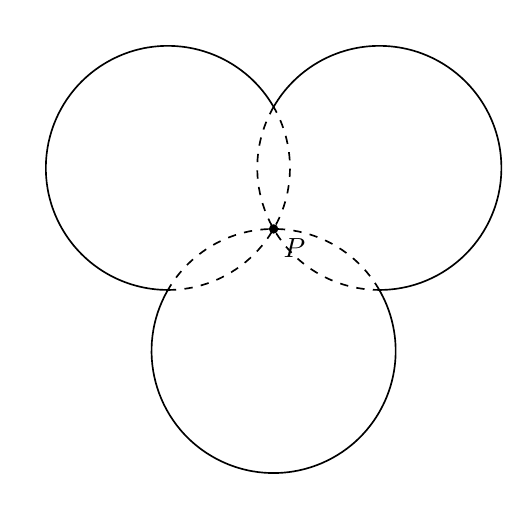
\begin{tikzpicture}[scale=1.55, semithick]
  \coordinate (P) at (0,0);
  \coordinate (O1) at (-0.8660254,0.5);
  \coordinate (O2) at (0.8660254,0.5);
  \coordinate (O3) at (0,-1);

  % 封闭曲线 C：三段不含 P 的外侧弧（实线）
  \draw (O1) ++(30:1) arc[start angle=30, end angle=270, radius=1];
  \draw (O2) ++(-90:1) arc[start angle=-90, end angle=150, radius=1];
  \draw (O3) ++(150:1) arc[start angle=150, end angle=390, radius=1];

  % 三个圆上含 P 的内侧弧（原页虚线）
  \draw[dashed] (O1) ++(270:1) arc[start angle=270, end angle=390, radius=1];
  \draw[dashed] (O2) ++(150:1) arc[start angle=150, end angle=270, radius=1];
  \draw[dashed] (O3) ++(30:1) arc[start angle=30, end angle=150, radius=1];

  % 公共点 P 及标注
  \fill (P) circle (1.1pt);
  \node[below right] at (P) {$P$};
\end{tikzpicture}
\end{center}
\nopagebreak[4]
\end{question}
\endgroup
\gkpart{三、解答题}
\begin{question}
\gkti{16}已知 $\{a_n\}$ 是首项为 $19$，公差为 $-2$ 的等差数列，$S_n$ 为 $\{a_n\}$ 的前 $n$ 项和。

（1）求通项 $a_n$ 及 $S_n$；

（2）设 $\{b_n-a_n\}$ 是首项为 $1$，公比为 $3$ 的等比数列，求数列 $\{b_n\}$ 的通项公式及前 $n$ 项和 $T_n$。

\end{question}
\begin{question}
\gkti{17}在甲、乙等 $6$ 个单位参加的一次“唱读讲传”演出活动中，每个单位的节目集中安排在一起。若采用抽签的方式随机确定各单位的演出顺序（序号为 $1$，$2$，$\cdots$，$6$），求：

（1）甲、乙两单位的演出序号均为偶数的概率；

（2）甲、乙两单位的演出序号不相邻的概率。

\end{question}
\begin{question}
\gkti{18}设 $\triangle ABC$ 的内角 $A$，$B$，$C$ 的对边长分别为 $a$，$b$，$c$，且 $3b^2+3c^2-3a^2=4\sqrt2bc$。

（1）求 $\sin A$ 的值；

（2）求 $\dfrac{2\sin\left(A+\dfrac{\pi}{4}\right)\sin\left(B+C+\dfrac{\pi}{4}\right)}{1-\cos 2A}$ 的值。

\end{question}
\begin{question}
\gkti{19}已知函数 $f(x)=ax^3+x^2+bx$（其中常数 $a$，$b\in\mathbf R$），$g(x)=f(x)+f'(x)$ 是奇函数。

（1）求 $f(x)$ 的表达式；

（2）讨论 $g(x)$ 的单调性，并求 $g(x)$ 在区间 $[1,2]$ 上的最大值和最小值。

\Needspace{0.4\textheight}
\end{question}
\begingroup
\renewenvironment{question}{\Needspace{0.5\textheight}}{}
\begin{question}
\gkti{20}如图，四棱锥 $P-ABCD$ 中，底面 $ABCD$ 为矩形，$PA\perp$ 底面 $ABCD$，$PA=AB=\sqrt2$，点 $E$ 是棱 $PB$ 的中点。

（1）证明：$AE\perp$ 平面 $PBC$；

（2）若 $AD=1$，求二面角 $B-EC-D$ 的平面角的余弦值。
\nopagebreak[4]
\begin{center}% 2010 年重庆卷文科第 20 题：四棱锥 P-ABCD，底面 ABCD 为矩形，PA⊥底面，E 为棱 PB 的中点。
% 来源 PDF：普通高考/2010/2010重庆文.pdf，SHA-256 634c8ac529a6ea52305b2909eff8730888048b77d082897394bfda22cb3fe73b。
% 原页：第 2 页（A3 三栏）第 2 栏中部，书页码 580。
% 重绘依据：按原页图形比例量取顶点位置（以 BC=4 为单位长，近似）：
%   B(0,0)、C(4,0)、A(1.7,1.6)、D(5.3,1.6)、P(1.7,7.2)、E(0.85,3.6)，P 在 A 的正上方、E 为 PB 中点。
% 实线：BC、CD、PB、PC、PD、CE；虚线：PA、AB、AD、AC、AE、DE（与原页虚线段一一对应）。
% 原页在顶点 A 处画一个小叉表示该顶点被遮挡，此图照录。
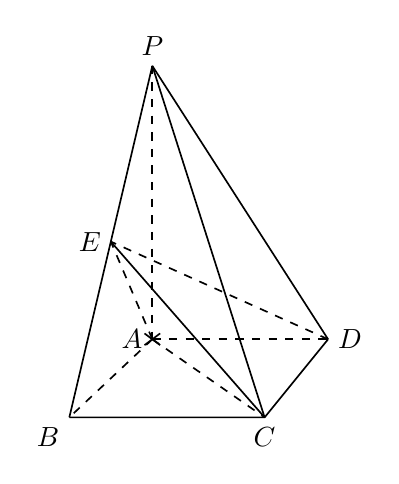
\begin{tikzpicture}[scale=0.62, semithick]
  \coordinate (B) at (0,0);
  \coordinate (C) at (4,0);
  \coordinate (A) at (1.7,1.6);
  \coordinate (D) at (5.3,1.6);
  \coordinate (P) at (1.7,7.2);
  \coordinate (E) at (0.85,3.6);

  % 可见棱
  \draw (B) -- (C) -- (D);
  \draw (P) -- (B);
  \draw (P) -- (C);
  \draw (P) -- (D);
  \draw (C) -- (E);

  % 被遮挡的棱
  \draw[dashed] (P) -- (A);
  \draw[dashed] (A) -- (B);
  \draw[dashed] (A) -- (D);
  \draw[dashed] (A) -- (C);
  \draw[dashed] (A) -- (E);
  \draw[dashed] (D) -- (E);

  % 原页在 A 处的遮挡叉号
  \draw[line width=0.6pt] (1.54,1.48) -- (1.86,1.72);
  \draw[line width=0.6pt] (1.54,1.72) -- (1.86,1.48);

  \node[above]       at (P) {$P$};
  \node[left]        at (E) {$E$};
  \node[left]        at (A) {$A$};
  \node[below left]  at (B) {$B$};
  \node[below]       at (C) {$C$};
  \node[right]       at (D) {$D$};
\end{tikzpicture}
\end{center}
\nopagebreak[4]
\Needspace{0.4\textheight}
\end{question}
\endgroup
\begingroup
\renewenvironment{question}{\Needspace{0.5\textheight}}{}
\begin{question}
\gkti{21}已知以原点 $O$ 为中心，$F(\sqrt5,0)$ 为右焦点的双曲线 $C$ 的离心率 $e=\dfrac{\sqrt5}{2}$。

（1）求双曲线 $C$ 的标准方程及其渐近线方程；

（2）如图，已知过点 $M(x_1,y_1)$ 的直线 $l_1$：$x_1x+4y_1y=4$ 与过点 $N(x_2,y_2)$（其中 $x_2\neq x_1$）的直线 $l_2$：$x_2x+4y_2y=4$ 的交点 $E$ 在双曲线 $C$ 上，直线 $MN$ 与两条渐近线分别交于 $G$、$H$ 两点，求 $\overrightarrow{OG}\cdot\overrightarrow{OH}$ 的值。
\nopagebreak[4]
\begin{center}% 2010 年重庆卷文科第 21 题：双曲线 C（中心 O，右焦点 F）与两条渐近线、直线 l1、l2、MN 的位置图。
% 来源 PDF：普通高考/2010/2010重庆文.pdf，SHA-256 634c8ac529a6ea52305b2909eff8730888048b77d082897394bfda22cb3fe73b。
% 原页：第 2 页（A3 三栏）第 3 栏中部，书页码 580。
% 重绘依据：按原页图形拓扑重绘，坐标取在本图自己的尺度上，并满足题设关系：
%   原点 O(0,0)；x 轴约 -1.5～7.4，y 轴约 -3.2～4.0；
%   双曲线只画右支 x=2√(1+y²)（原页即只画右支，线较粗）；
%   两条渐近线均自 O 向右上方、右下方画出（原页也不画左半段）；
%   取 E(3.61,-1.50) 在右支上，l1 过 M(-1.00,-1.27)，l2 过 N(1.80,0.42)；
%   MN 过 M、N（即 x_E x + 4y_E y = 4），与 y=x/2 交于 G(6.60,3.30)、与 y=-x/2 交于 H(0.61,-0.30)；
%   原页 M、N 为实心圆点，E、G、H 无圆点；E 为 l1、l2 的交点，不在 MN 上。
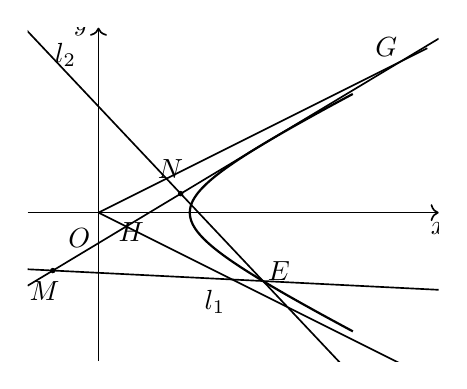
\begin{tikzpicture}[scale=0.58, semithick]
  \coordinate (O) at (0,0);
  \coordinate (M) at (-1.00,-1.268);
  \coordinate (N) at (1.80,0.416);
  \coordinate (E) at (3.606,-1.50);
  \coordinate (G) at (6.60,3.30);
  \coordinate (H) at (0.606,-0.303);

  \clip (-1.55,-3.25) rectangle (7.45,4.05);

  % 坐标轴
  \draw[->] (-1.55,0) -- (7.45,0) node[below] {$x$};
  \draw[->] (0,-3.25) -- (0,4.05) node[left] {$y$};

  % 双曲线右支 x^2/4-y^2=1
  \draw[thick] plot[domain=-2.60:2.60, samples=140, variable=\y]
    ({2*sqrt(1+\y*\y)}, \y);

  % 渐近线 y=±x/2（只画右半）
  \draw (O) -- (7.20,3.60);
  \draw (O) -- (7.20,-3.60);

  % l1（过 M、E）、l2（过 N、E）、MN（过 M、N）
  \draw (-1.55,-1.24) -- (7.45,-1.69);
  \draw (-1.60,4.023) -- (5.40,-3.404);
  \draw (-1.55,-1.60) -- (7.45,3.81);

  % 点 M、N 处实心圆点
  \fill (M) circle (1.7pt);
  \fill (N) circle (1.7pt);

  % 文字（位置照原页）
  \node at (-0.72,3.45) {$l_2$};
  \node at (2.55,-1.95) {$l_1$};
  \node at (-0.42,-0.55) {$O$};
  \node at (-1.18,-1.72) {$M$};
  \node at (1.58,0.95) {$N$};
  \node at (6.30,3.62) {$G$};
  \node at (0.72,-0.42) {$H$};
  \node at (3.95,-1.28) {$E$};
\end{tikzpicture}
\end{center}
\nopagebreak[4]

\end{question}
\endgroup
\end{document}
